\subsection{An Architecture for Believable Socially Aware Agents}
\label{sec:dorgoly}
Dorgoly's work presents a novel architecture to address believability in \ac{NPC}s with special atention to the social capabilities of the \ac{NPC} \cite{dorgoly:social-agents}.

This is done by introducing a role based architecture and using role variables to customize agent processes such as planning and emotion appraisal to achieve the agent's goals (check Dorgoly's agent architecture in Fig. \ref{fig:believable-social-agents-architecture}).

\begin{figure}
  \centering
    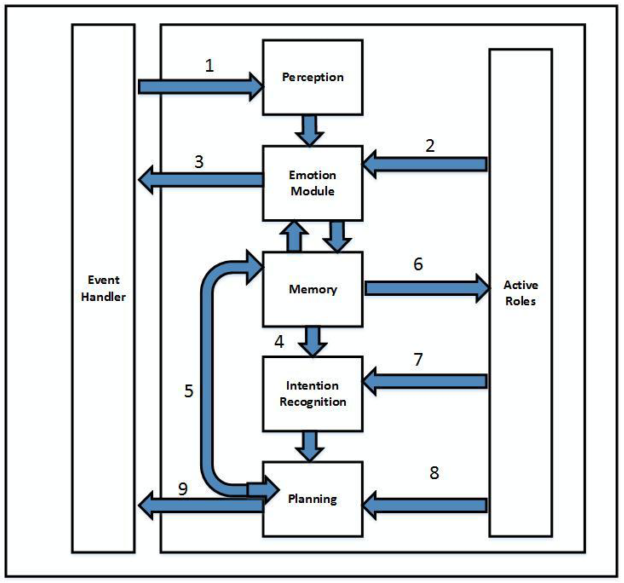
\includegraphics[width=.75\textwidth]{believable-social-agents-architecture}
  \caption{Dorgoly's proposed architecture.}
  \label{fig:believable-social-agents-architecture}
\end{figure}

The agent process starts by receiving a message from the world.
The event will be appraised by emotional rules; active roles that represent the agent social context affect this appraisal process.
The received event may be saved in the Memory; furthermore it may cause the agent to update its original plan.
Intention recognition selects a goal and planning generates a plan for this goal.

\begin{description}
\item \textbf{Perception} This module is responsible for parsing the events of the world and pass them to the Emotion Module
\item \textbf{Emotion Module} The Emotion Module will work with the Memory in order to appraise a given event with general emotion rules.
However, if the given event confirms a goal state achievement it cannot be appraised simply by applying emotion rules.
By working together with the Memory, the Emotion Module will then appraise the event accordingly.
This appraisal will be applied to emotion reactive rules and may trigger non-planned impulsive actions (e.g. if the agent fails to achieve a long term goal it may burst into tears).
Finally, the Emotional Module will update the Emotional State of the agent with the current appraised emotion.
\item \textbf{Memory} The Memory stores past events, the active plan and a representation of other agent's minds (\textit{theory of mind}).
After the appraisal of an event, the event and appraised emotion will be stored in the agents' Memory and the profiles of the other agents are updated in the TOM module of the Memory.
The Memory is also responsible for keeping track of the agent planning and validating the next action in the plan.
In the event of an invalid action, the agent must make a new plan.
If the plan has finished the memory must inform the intention recognition to set a new goal for the agent.
\item \textbf{Intention Recognition} This module processes the agent's active roles and sets the agent intention on the most important goal.
\item \textbf{Planning Module} The Planning module receives the agent's goal and comes up to a plan to achieve it.
\item \textbf{Active Role} A role has a set of personality traits, beliefs, and goals that represent the agents' social context.
A role is defined as the relationship of one person to another person, group or object.
It formalizes an agent's relationship with its environment and with other agents, including other agents' expectations based on this relationship.
Essentially, a role specifies how the agent should act. 
\end{description}

Using Dorgoly's architecture, we can create agents with qualities such as being reactive, being responsive, and having the presence of a goal and personality.
Has we have discussed in \ref{sec:social-agents}, agents' actions must be social by themselves, and this architecture provides just that, by using roles to influence its actions.
